\section{Experimentación} \label{section:Experimentation}

Con el objetivo de comprobar la viabilidad y funcionamiento del prototipo implementado se propone la evaluación 
de su comportamiento ante dos escenarios de prueba. Los experimentos se dividen en fases. La primera fase verifica 
la correctitud del proceso de exploración efectuado por el Crawler y creación de la base de datos de Neo4j en el  
Catálogo de Datos para la fuente de datos de turno. La segunda fase consiste en la creación 
del grafo de join y \'arboles de join. La tercera fase consiste en la generación de las consultas dado una 
definición de esquema 
estrella mediante un script del DSL y la selección de los joins efectuada por el usuario. La cuarta fase y \'ultima 
es la validación de las consultas generadas 
mediante la creación manual de un pipeline de población a partir de las mismas y su ejecución. Todos los archivos que intervienen 
en el proceso de experimentación se encuentran en la carpeta \textbf{experiments} en el directorio raíz del proyecto. 
Cada experimento posee su propia carpeta en las cuales existen tres scripts de python y un scripts del DSL que constituye 
la definición del esquema estrella a poblar. Los scripts de python tienen el mismo nombre en ambas carpetas de experimentación, 
\textbf{create.py}, \textbf{populate.py}, \textbf{pipeline.py}. El primero se encarga de 
crear la base de datos correspondiente al escenario de ventas minoristas descrito anteriormente. El segundo se 
encarga de poblar dicha base de datos. El tercero es la implementación de un pipeline de población utilizando 
las consultas generadas. Los scripts utilizan las librerías de python SQLAlchemy, Psycopg2 y Faker para llevar a 
cabo sus tareas. En particular, la biblioteca de python Faker proporciona facilidades para la generación de información, 
la cual es utilizada para poblar las bases de datos de prueba. A continuación se describen 
los detalles de los experimentos.

\subsection{Ambiente de experimentación}

\subsubsection{Equipo}

Se utilizó una computadora portátil con un procesador Intel(R) Core(TM) i7-11370H 11th Gen @ 3.30GHz, 16GB de 
memoria RAM y sistema operativo Windows 11 Home 23H2.

\subsubsection{Docker}

Se utilizó Docker para simular el traspaso de datos por red entre la aplicación, el Catálogo de Datos y 
los servidores de bases de datos fuente y destino. Se crea una imagen de la aplicación basada en python:3.10, con el 
nombre \textbf{autoetl}. 
Con el archivo \textbf{docker-compose.yml} se inicializan todos los contenedores que intervienen en el proceso 
de experimentación. Los servidores de bases de datos fuente y destino son contenedores de PostgreSQL llamados 
\textbf{db} y \textbf{target} respectivamente. El Catálogo de Datos es un contenedor de Neo4j con nombre 
\textbf{data\_catalog}. La aplicación implementada yace en un contenedor de la imagen creada \textbf{autoetl}. 
Por \'ultimo, con el objetivo de visualizar los resultados del proceso de población se añade al ambiente un 
contenedor de \textbf{pgadmin4}, el cual proporciona una herramienta para la visualización de bases de datos 
de PostgreSQL.

\subsection{Experimento 1: Escenario de ventas minoristas}

Este escenario se basa en \textbf{Retail Sales} expuesto en el capítulo 2
de \cite{kimball2011data}. 

Una red de tiendas cuenta con sucursales distribuidas en varias provincias del país. Estas tiendas se encuentran ubicadas 
en diferentes barrios de los municipios de cada provincia. Las tiendas se dividen en departamentos y cada uno vende 
una serie de productos. Se almacenan los detalles de las transacciones realizadas, es decir, las ventas. Para cada venta, se guarda 
el producto vendido, la tienda en la que se realizó, la fecha de la transacción, la cantidad vendida y el monto pagado.
La figura \ref{fig:retail-transactional} muestra las tablas del sistema transaccional y la relación entre ellas.

\begin{figure}[ht]
    \centering
    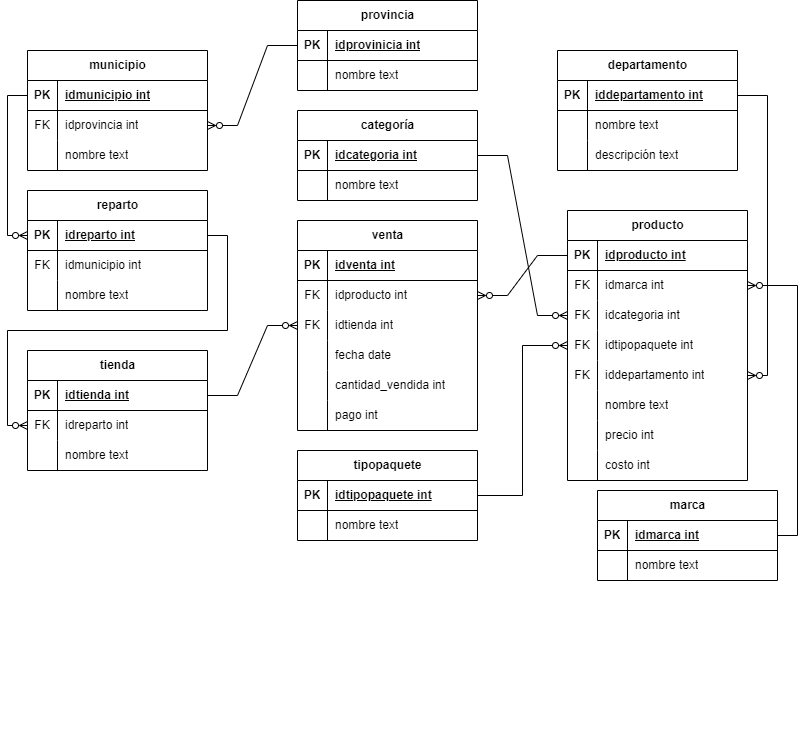
\includegraphics[scale=0.5]{Graphics/retailSales-Transactional.drawio.png}
    \caption{Sistema Transaccional: Ventas Minoristas}
    \label{fig:retail-transactional}
  \end{figure}

Los archivos que intervienen en este experimento se encuentran en la carpeta \textbf{retail\_sales} del 
directorio \textbf{experiments}. La definición del esquema estrella a poblar se encuentra en el archivo 
\textbf{retailsales.txt}, el listado de código \ref{retailsalesstar} muestra su contenido. La figura \ref{fig:retail-Warehouse} muestra la composición de las 
tablas de dimensión y de hechos del esquema estrella propuesto. 

\begin{lstlisting}[label={retailsalesstar}, caption={Definici\'on del esquema estrella del almacén de datos asociado al escenario ventas minoristas}]
  dimension tienda {
  tienda: idtienda PK
  tienda:nombre
  reparto:nombre as reparto
  municipio:nombre as municipio 1
  provincia:nombre as provincia 2
  }

  dimension producto {
  producto:idproducto PK
  marca:nombre as marca
  categoria:nombre as categoria
  tipopaquete:nombre as paquete
  departamento:nombre as departamento
  departamento:descripcion as descripcion
  producto:nombre as producto
  producto:precio
  producto:costo
  }

  dimension fecha {
  venta:fecha PK
  venta:week_day(fecha) str as Dia
  venta:month_str(fecha) str as Mes 1
  }

  fact venta {
  self:idventa PK serial
  venta:idproducto FK to producto.idproducto 
  venta:idtienda FK to tienda.idtienda
  venta:fecha FK to fecha.fecha
  venta:sum(cantidad_vendida) as cantidad_vendida_total
  venta:sum(pago) as importe_total
  producto:Costo * venta:sum(cantidad_vendida) int as coste_total
  venta:sum(pago) - producto:Costo * venta:sum(cantidad_vendida) int as ganancia 
  }
\end{lstlisting}

\begin{figure}
    \centering
    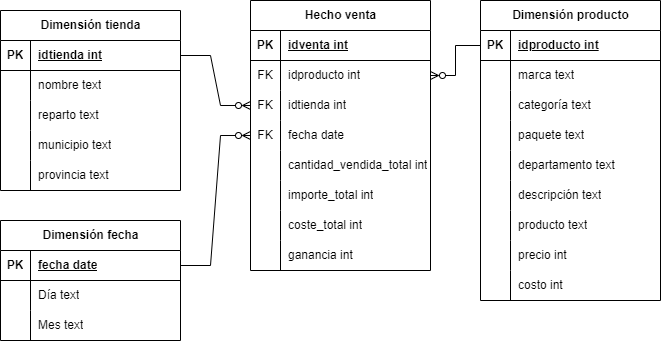
\includegraphics[scale=0.5]{Graphics/retailSales-Data Warehouse.drawio.png}
    \caption{Almacén de Datos: Ventas Minoristas}
    \label{fig:retail-Warehouse}
\end{figure}

\subsubsection{Fase 1: Exploraci\'on del Crawler y creaci\'on de la base de datos de Neo4j}

Para el esquema de base de datos de la figura \ref{fig:retail-transactional} la base de datos de Neo4j derivada a 
partir de los datos recopilados por el Crawler se muestra en la figura \ref{fig:catalogexp1}.

\begin{figure}
  \centering
  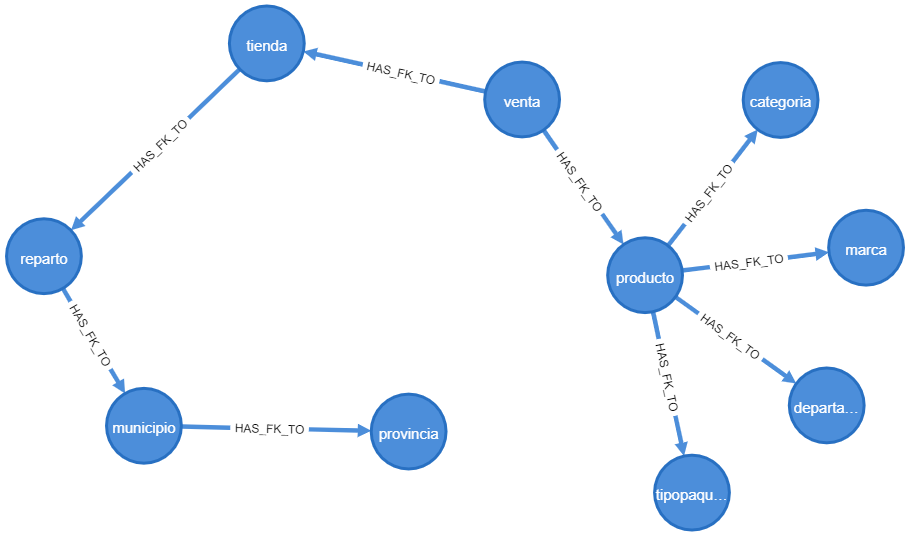
\includegraphics[scale=0.4]{Graphics/graph (1).png}
  \caption{Grafo de Neo4j para el esquema de ventas minoristas}
  \label{fig:catalogexp1}
\end{figure}

\subsubsection{Fase 2: Creaci\'on del grafo de join y \'arboles de join}

A partir de la base de datos de Neo4j obtenido en la fase 1 se computan el grafo de join y el \'arbol de 
join que se muestran en la figura \ref{fig:graphjoin1} y en la figura \ref{fig:jointree1} respectivamente. Para este caso, 
el \'arbol de join es \'unico y coincide  con el grafo de join debido a que el esquema de bases de datos de 
las ventas minoristas no presenta ambigüedades.

\begin{figure}
  \centering
  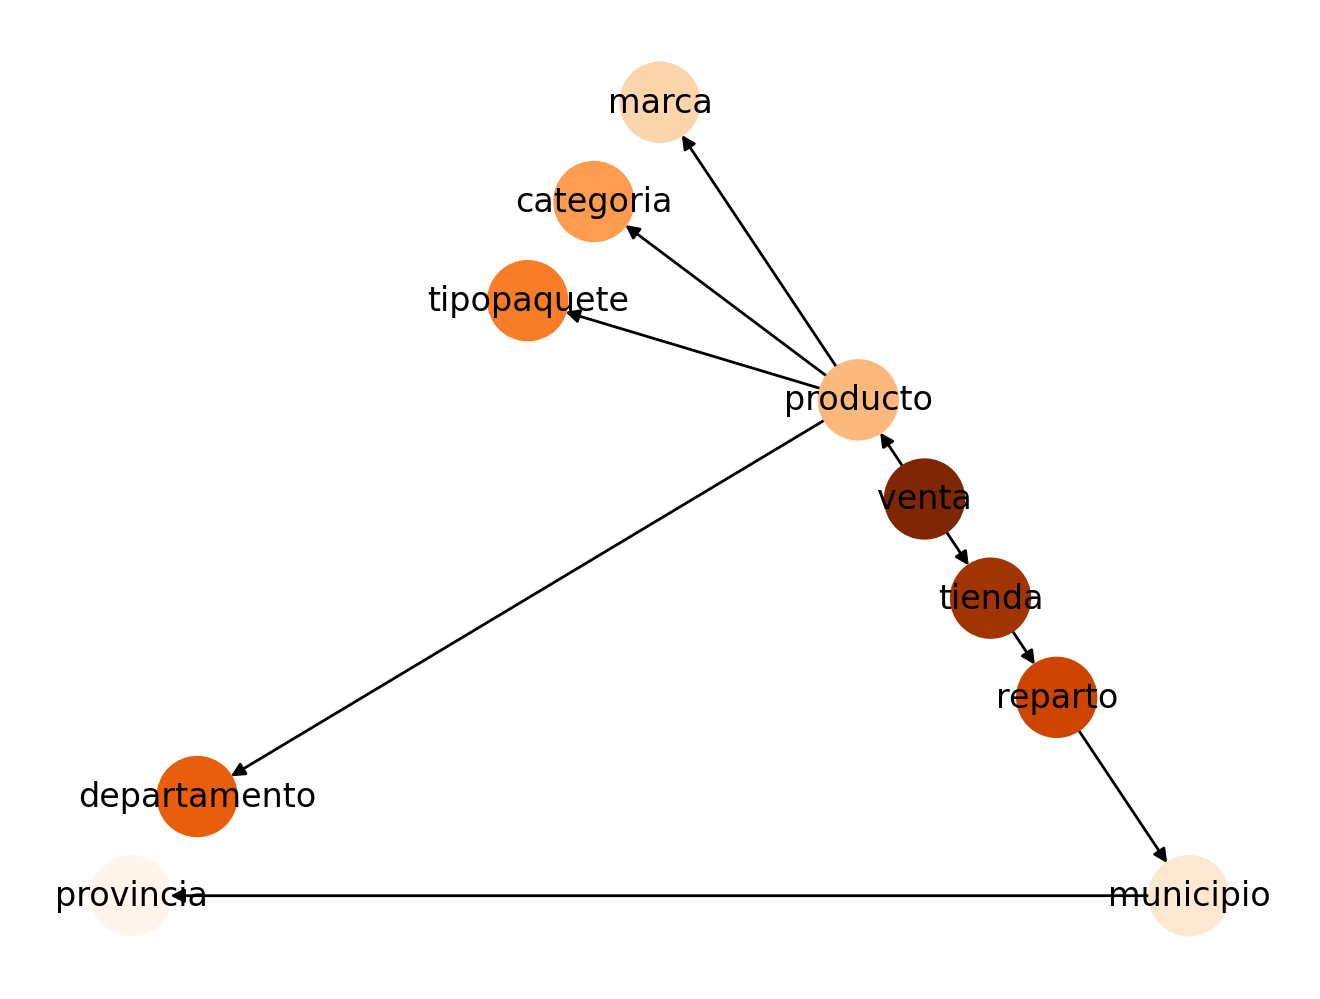
\includegraphics[scale=0.6]{Graphics/joingraph1.png}
  \caption{Grafo de join para el esquema de ventas minoristas}
  \label{fig:graphjoin1}
\end{figure}

\begin{figure}
  \centering
  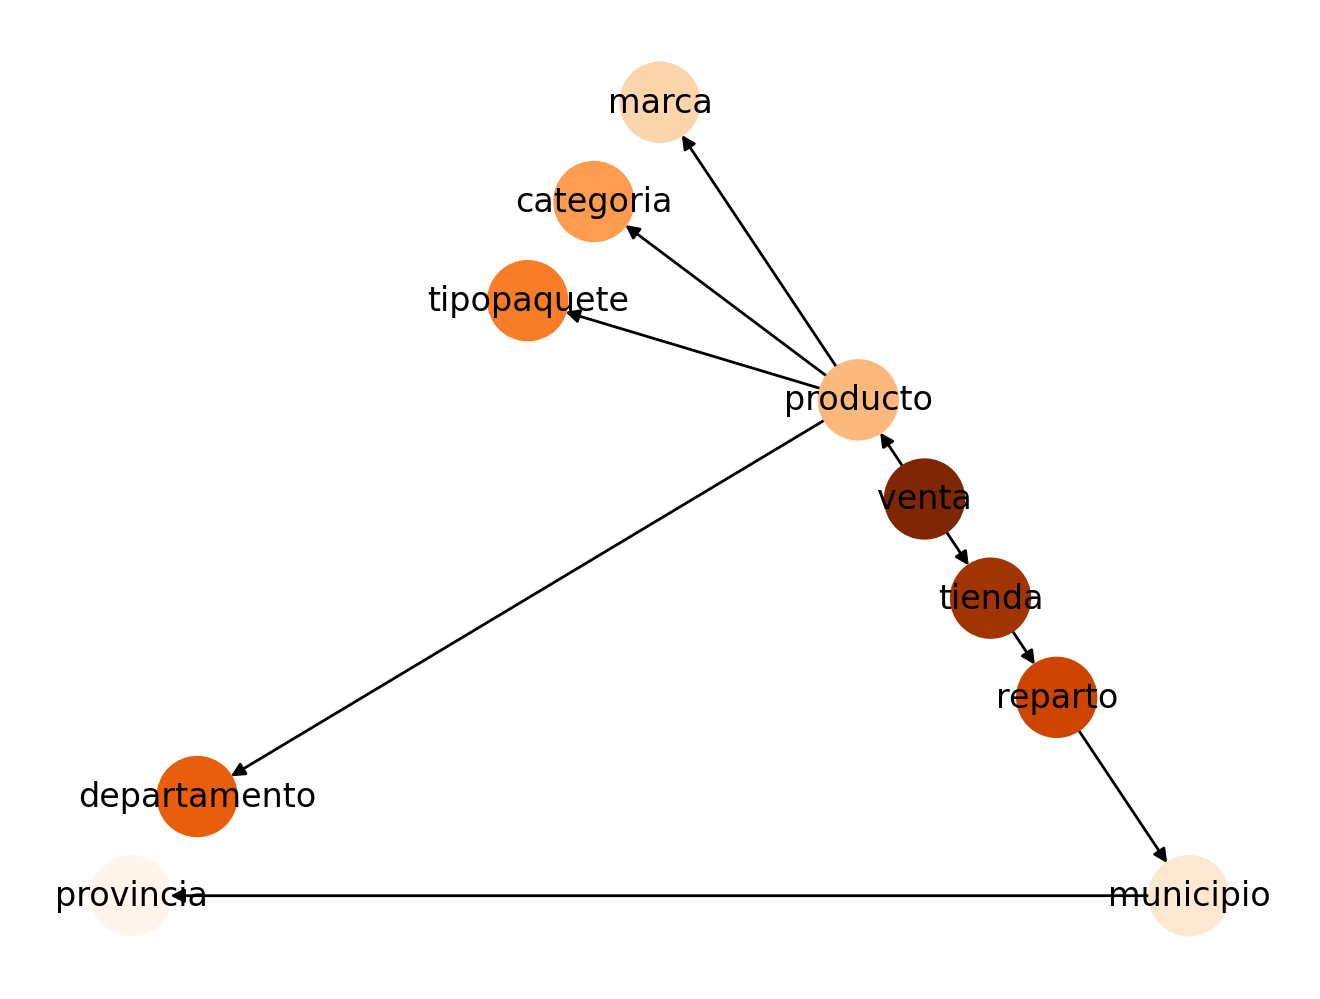
\includegraphics[scale=0.6]{Graphics/jointree1.png}
  \caption{\'Arbol de join para el esquema de ventas minoristas}
  \label{fig:jointree1}
\end{figure}

\subsubsection{Fase 3: Generaci\'on de las consultas}

La selección de los joins por parte del usuario se efectúa a través de la interfaz de usuario. 
Como solo hay un \'arbol de join hay una \'unica opción de join para 
cada tabla del esquema estrella. El listado de código \ref{joinselectexp1} muestra los joins 
computados a partir del \'arbol de join mostrado en la fase 2 y de la definición del esquema estrella 
presente en \textbf{retailsales.txt}.

\begin{lstlisting}[label={joinselectexp1}, caption={Joins computados para el experimento 1}, language={sql}]
  -- Joins for tienda
  1: tienda JOIN reparto ON tienda.idreparto = reparto.idreparto 
     JOIN municipio ON reparto.idmunicipio = municipio.idmunicipio 
     JOIN provincia ON municipio.idprovincia = provincia.idprovincia

  -- Joins for producto
  1: producto JOIN departamento ON producto.iddepartamento = departamento.iddepartamento 
     JOIN tipopaquete ON producto.idtipopaquete = tipopaquete.idtipopaquete 
     JOIN categoria ON producto.idcategoria = categoria.idcategoria 
     JOIN marca ON producto.idmarca = marca.idmarca

  -- Joins for fecha
  1: venta

  -- Joins for venta
  1: venta JOIN producto ON venta.idproducto = producto.idproducto
  
\end{lstlisting}

El listado de código \ref{quercreateexp1} muestra las consultas de creación y el listado de código 
\ref{selectexp1} muestra las consultas de selección, generadas a partir de los joins computados en 
la fase previa.

\begin{lstlisting}[label={quercreateexp1}, caption={Consultas de creaci\'on generadas para el experimento 1}, language={sql}]
  -- Creation query's
  CREATE TABLE IF NOT EXISTS fecha (
  fecha DATE, 
  Dia TEXT, 
  Mes TEXT, 
  PRIMARY KEY (fecha)
  );

  CREATE TABLE IF NOT EXISTS producto (
  idproducto INT, 
  marca TEXT, 
  categoria TEXT, 
  paquete TEXT, 
  departamento TEXT, 
  descripcion TEXT, 
  producto TEXT, 
  precio INT, 
  costo INT, 
  PRIMARY KEY (idproducto)
  );

  CREATE TABLE IF NOT EXISTS tienda (
  idtienda INT, 
  nombre TEXT, 
  reparto TEXT, 
  municipio TEXT, 
  provincia TEXT, 
  PRIMARY KEY (idtienda)
  );

  CREATE TABLE IF NOT EXISTS venta (
  idventa serial, 
  idproducto INT, 
  idtienda INT, 
  fecha DATE, 
  cantidad_vendida_total INT, 
  importe_total INT, 
  coste_total INT, 
  ganancia INT, 
  PRIMARY KEY (idventa), 
  FOREIGN KEY (idproducto) REFERENCES producto (idproducto), 
  FOREIGN KEY (idtienda) REFERENCES tienda (idtienda), 
  FOREIGN KEY (fecha) REFERENCES fecha (fecha), 
  UNIQUE(idproducto, idtienda, fecha)
  );

  -- level metadata
  CREATE TABLE IF NOT EXISTS level_metadata (
                                  table_name TEXT,
                                  attribute_name TEXT,
                                  level INT,
                                  PRIMARY KEY (table_name, attribute_name, level));

  INSERT INTO level_metadata VALUES('tienda', 'idtienda', 0);
  INSERT INTO level_metadata VALUES('tienda', 'nombre', 0);
  INSERT INTO level_metadata VALUES('tienda', 'reparto', 0);
  INSERT INTO level_metadata VALUES('tienda', 'municipio', 1);
  INSERT INTO level_metadata VALUES('tienda', 'provincia', 2);
  INSERT INTO level_metadata VALUES('producto', 'idproducto', 0);
  INSERT INTO level_metadata VALUES('producto', 'marca', 0);
  INSERT INTO level_metadata VALUES('producto', 'categoria', 0);
  INSERT INTO level_metadata VALUES('producto', 'paquete', 0);
  INSERT INTO level_metadata VALUES('producto', 'departamento', 0);
  INSERT INTO level_metadata VALUES('producto', 'descripcion', 0);
  INSERT INTO level_metadata VALUES('producto', 'producto', 0);
  INSERT INTO level_metadata VALUES('producto', 'precio', 0);
  INSERT INTO level_metadata VALUES('producto', 'costo', 0);
  INSERT INTO level_metadata VALUES('fecha', 'fecha', 0);
  INSERT INTO level_metadata VALUES('fecha', 'Dia', 0);
  INSERT INTO level_metadata VALUES('fecha', 'Mes', 1);
  INSERT INTO level_metadata VALUES('venta', 'idventa', 0);
  INSERT INTO level_metadata VALUES('venta', 'idproducto', 0);
  INSERT INTO level_metadata VALUES('venta', 'idtienda', 0);
  INSERT INTO level_metadata VALUES('venta', 'fecha', 0);
  INSERT INTO level_metadata VALUES('venta', 'cantidad_vendida_total', 0);
  INSERT INTO level_metadata VALUES('venta', 'importe_total', 0);
  INSERT INTO level_metadata VALUES('venta', 'coste_total', 0);
  INSERT INTO level_metadata VALUES('venta', 'ganancia', 0);
\end{lstlisting}

\begin{lstlisting}[label={selectexp1}, caption={Consultas de selecci\'on generadas para el experimento 1}, language={sql}]
  -- Selection for fecha
  SELECT DISTINCT venta.fecha, to_char(venta.fecha, 'Day') AS Dia, to_char(venta.fecha, 'Month') AS Mes
  FROM venta;

  -- Selection for producto
  SELECT DISTINCT producto.idproducto, marca.nombre AS marca, categoria.nombre AS categoria, tipopaquete.nombre AS paquete, departamento.nombre AS departamento, departamento.descripcion AS descripcion, producto.nombre AS producto, producto.precio, producto.costo
  FROM producto
  JOIN departamento ON producto.iddepartamento = departamento.iddepartamento
  JOIN tipopaquete ON producto.idtipopaquete = tipopaquete.idtipopaquete
  JOIN categoria ON producto.idcategoria = categoria.idcategoria
  JOIN marca ON producto.idmarca = marca.idmarca;

  -- Selection for tienda
  SELECT DISTINCT tienda.idtienda, tienda.nombre, reparto.nombre AS reparto, municipio.nombre AS municipio, provincia.nombre AS provincia
  FROM tienda
  JOIN reparto ON tienda.idreparto = reparto.idreparto
  JOIN municipio ON reparto.idmunicipio = municipio.idmunicipio
  JOIN provincia ON municipio.idprovincia = provincia.idprovincia;

  -- Selection for venta
  SELECT DISTINCT venta.idproducto, venta.idtienda, venta.fecha, SUM(venta.cantidad_vendida) AS cantidad_vendida_total, SUM(venta.pago) AS importe_total, producto.Costo*SUM(venta.cantidad_vendida) AS coste_total, SUM(venta.pago)-producto.Costo*SUM(venta.cantidad_vendida) AS ganancia
  FROM venta
  JOIN producto ON venta.idproducto = producto.idproducto
  GROUP BY venta.idproducto,venta.idtienda,venta.fecha,producto.Costo;
\end{lstlisting}

\subsubsection{Fase 4: Creaci\'on manual del pipeline y poblaci\'on del almac\'en de datos}

El pipeline creado se encuentra en la ruta \textbf{experiments/retail\_sales} con el nombre de 
\textbf{pipeline.py}. Este script utiliza las consultas generadas ejecutando su código utilizando 
Psycopg2.

La figura \ref{fig:fullpg1} muestra el estado del servidor de bases de datos \textbf{target} luego de la ejecución 
del pipeline. La figura muestra como efectivamente 
se han creado y poblado todas la tablas del esquema estrella definido.

\begin{figure}
  \centering
  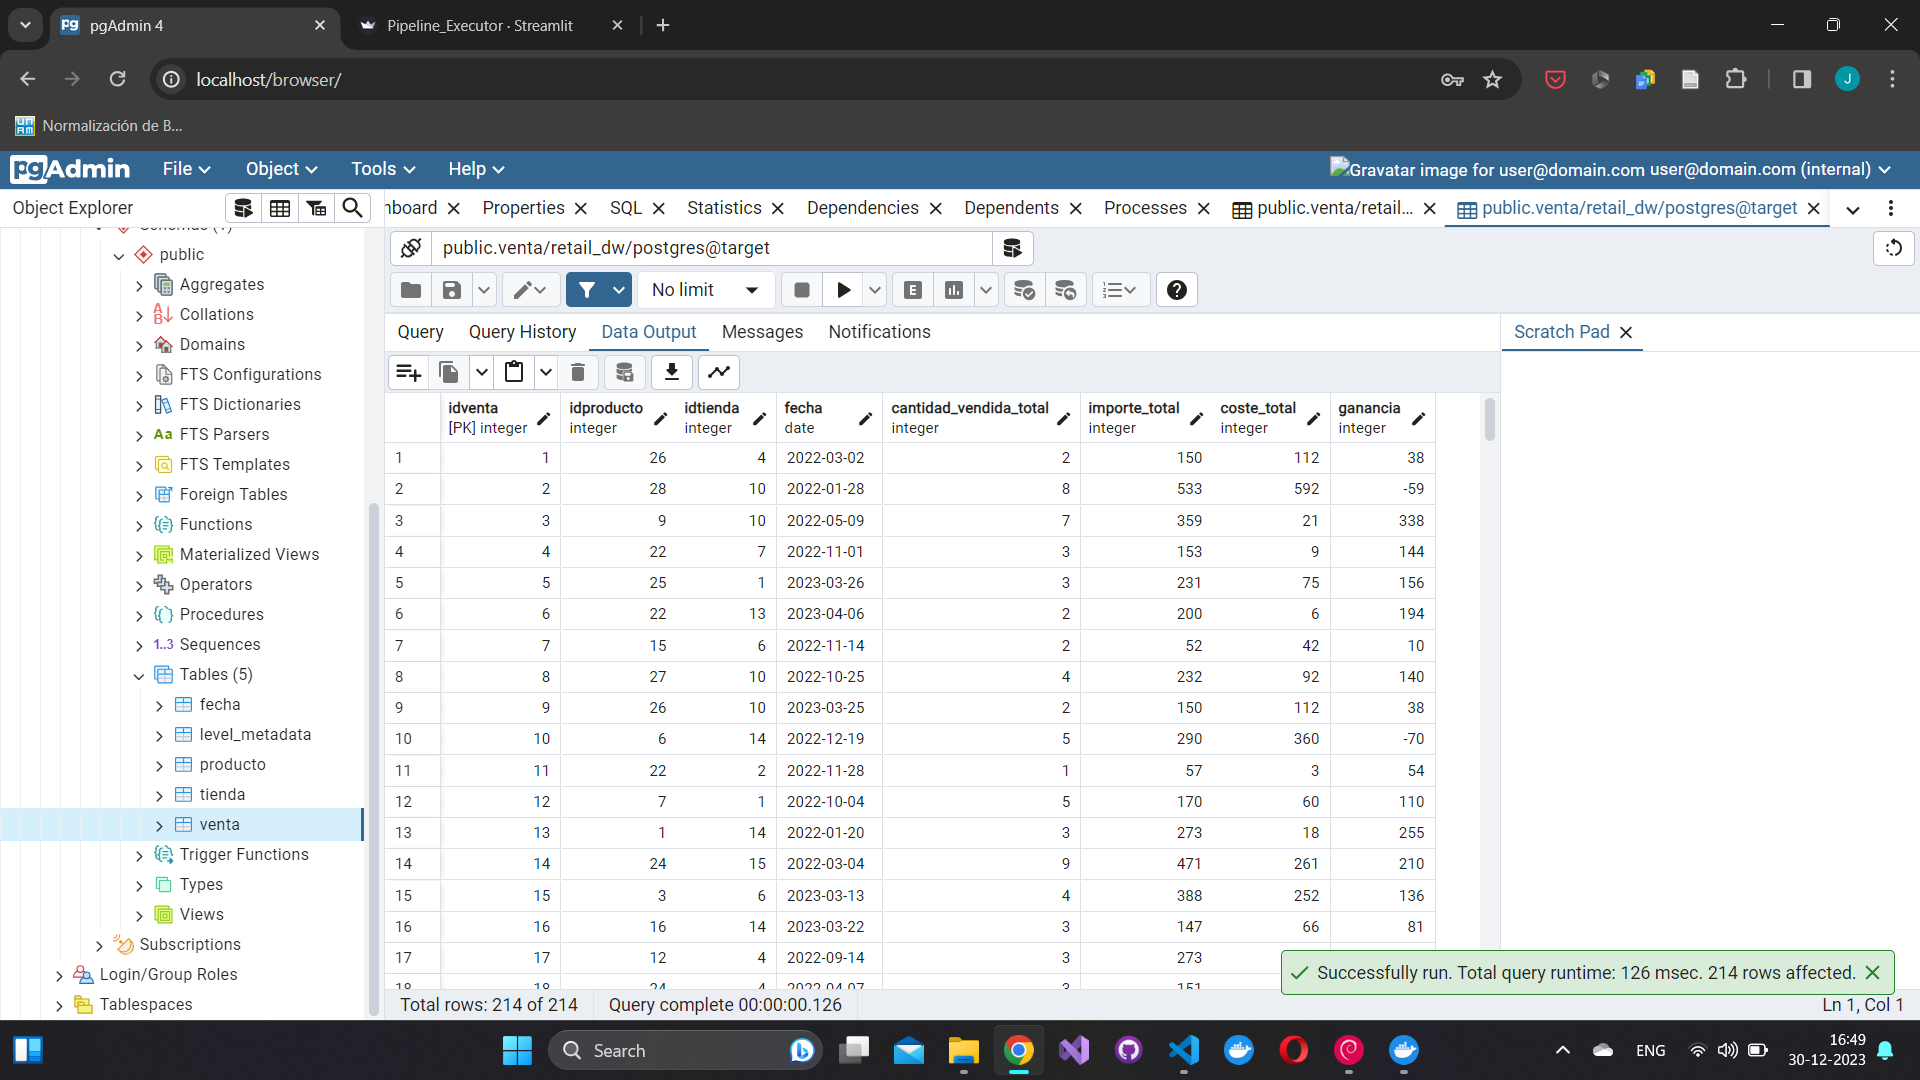
\includegraphics[scale=0.4]{Graphics/fullpgadmin1.png}
  \caption{Almacén de datos poblado asociado al escenario de ventas minoristas}
  \label{fig:fullpg1}
\end{figure}


\subsection{Experimento 2: Escenario TPCH}

Este escenario est\'a inspirado en el escenario de prueba TPCH\footnote{https://www.tpc.org/tpch/}, ampliamente 
utilizada para probar soluciones de bases de datos e Inteligencia de Negocios. Los scripts que participan 
en el proceso de creación y población de la base de datos de prueba TPCH se encuentran en la ruta 
\textbf{experiments/tpch}. La especificación del esquema estrella del almacén de datos a poblar se encuentra 
en el script del DSL \textbf{tpch.txt}, el listado de código \ref{tpchstar} muestra su contenido.  A continuación se describe el escenario que modela la base de datos.

\begin{lstlisting}[label={tpchstar}, caption={Definici\'on del esquema estrella del almacén de datos asociado al escenario TPCH}]
  dimension supplier {
    supplier: s_suppkey PK as suppkey
    supplier: s_name as name
    supplier: s_phone as phone
    supplier: s_address as address
    nation: n_name as nation
    region: r_name as region 1
  }

  dimension part {
      part: p_partkey PK
      part: p_name as name
      part: p_brand as brand
      part: p_size
      part: p_retailprice
  }

  dimension order_date {
      orders: o_orderdate PK as o_date
      orders:week_day(o_orderdate) str as day
      orders:month_str(o_orderdate) str as month 1
  }

  fact lineitem {
      self: linenumber PK serial as lnumber
      lineitem: l_partkey FK to part.p_partkey as partkey
      lineitem: l_suppkey FK to supplier.suppkey as supplierkey
      orders: o_orderdate FK to order_date.o_date as order_date
      lineitem: sum(l_payment) as totalpayment
      lineitem: sum(l_quantity) as totalquantity
      lineitem: sum(l_payment) - (lineitem: sum(l_quantity) * partsupp:ps_supplycost) - (lineitem: sum(l_quantity) * part:p_retailprice) numeric as earnings
  }
\end{lstlisting}

Una distribuidora vende piezas de varios suministradores. Distintos suministradores pueden 
producir la misma pieza. Los clientes de la suministradora realizan \'ordenes de compra 
de piezas de determinados suministradores. La figura  muestra el esquema de bases de datos 
del escenario TPCH. La figura \ref{fig:transactionaltpch} muestra el esquema de base de datos 
del escenario descrito.

\begin{figure}
  \centering
  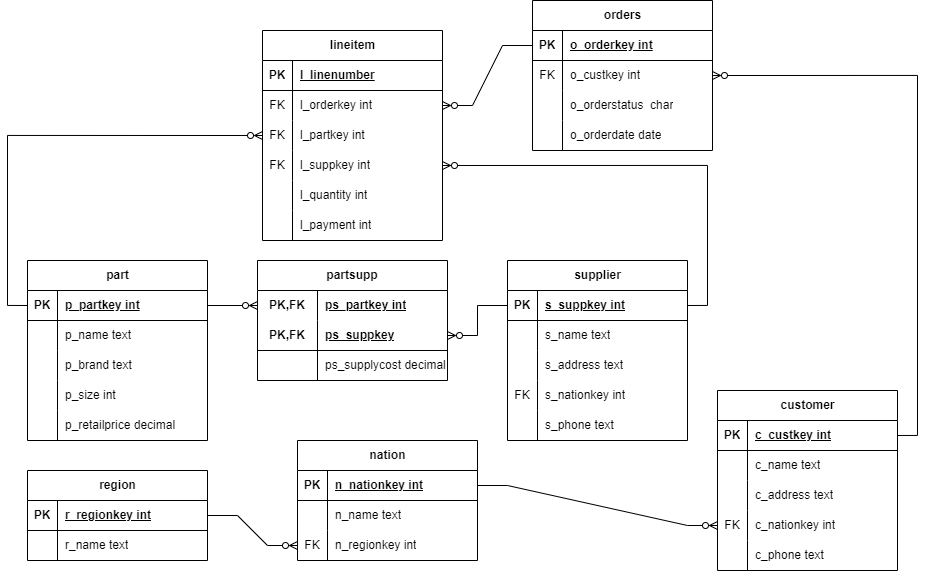
\includegraphics[scale=0.5]{Graphics/tpch-tpch-transactional.drawio (4).png}
  \caption{Esquema de la base de datos TPCH}
  \label{fig:transactionaltpch}
\end{figure}

La figura \ref{fig:warehousetpch} muestra el almacén de datos \textbf{tpch\_dw} que se poblar\'a a partir de los 
datos de la base de datos \textbf{TPCH}.

\begin{figure}
  \centering
  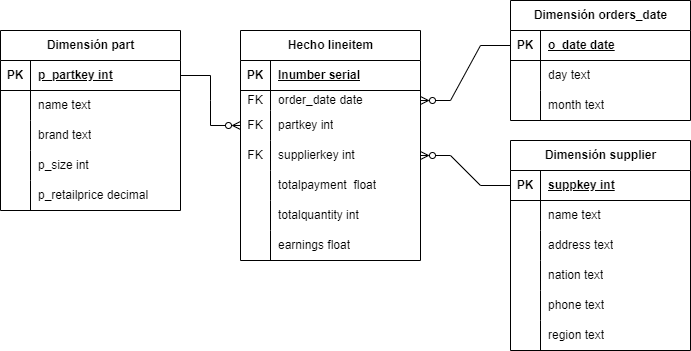
\includegraphics[scale=0.5]{Graphics/tpch-tpch-warehouse.drawio.png}
  \caption{Almacén de datos tpch\_dw}
  \label{fig:warehousetpch}
\end{figure}

\subsubsection{Fase 1: Exploraci\'on del Crawler y creaci\'on de la base de datos de Neo4j}

Para el esquema de base de datos de la figura \ref{fig:transactionaltpch} la base de datos de Neo4j derivada a 
partir de los datos recopilados por el Crawler se muestra en la figura \ref{fig:catalogexp2}.

\begin{figure}
  \centering
  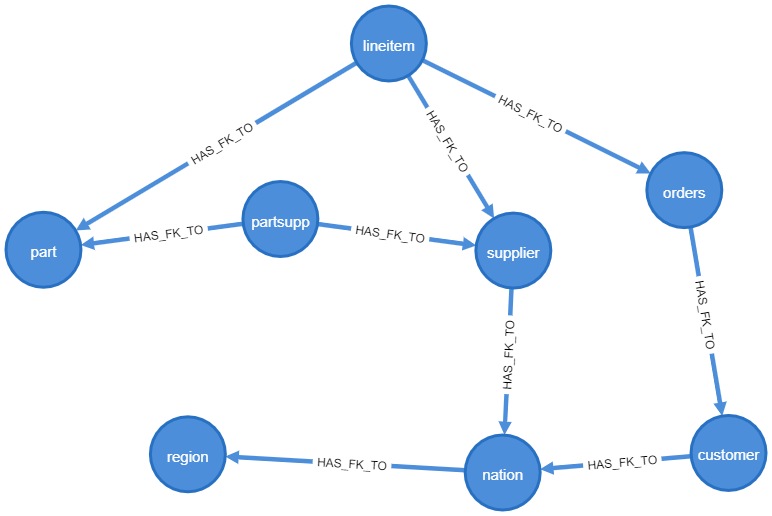
\includegraphics[scale=0.4]{Graphics/graph (2).png}
  \caption{Grafo de Neo4j para el esquema de TPCH}
  \label{fig:catalogexp2}
\end{figure}

\subsubsection{Fase 2: Creaci\'on del grafo de join y \'arboles de join}

A partir de la base de datos de Neo4j obtenido en la fase 1 se computan el grafo de join y los \'arboles de 
join que se muestran en la figura \ref{fig:graphjoin2} y en la figura \ref{fig:jointree2} respectivamente. 
N\'otese como en TPCH no existe una relaci\'on directa entre las tablas \textbf{Lineitem} y \textbf{PartSupplier}, 
sin embargo en el grafo de join se incluye un arco entre ellos dado que cumplen con el criterio expuesto 
en el cap\'itulo \ref{chapter:proposal} para la formaci\'on de arcos entre dos nodos del grafo de join.

\begin{figure}
  \centering
  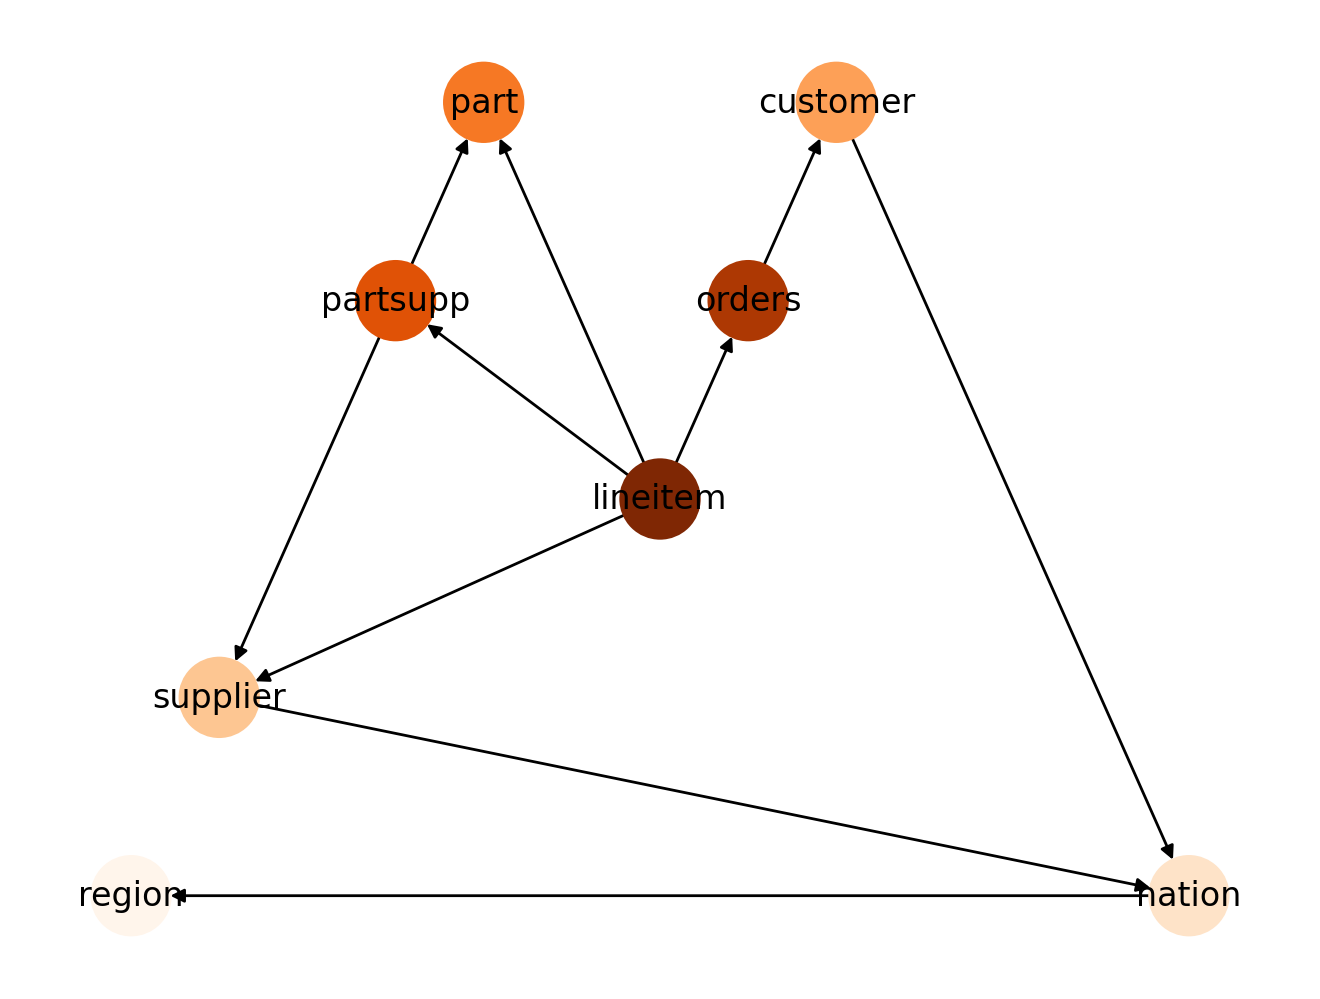
\includegraphics[scale=0.6]{Graphics/joingraph2.png}
  \caption{Grafo de join para el esquema de TPCH}
  \label{fig:graphjoin2}
\end{figure}

\begin{figure}
  \centering
  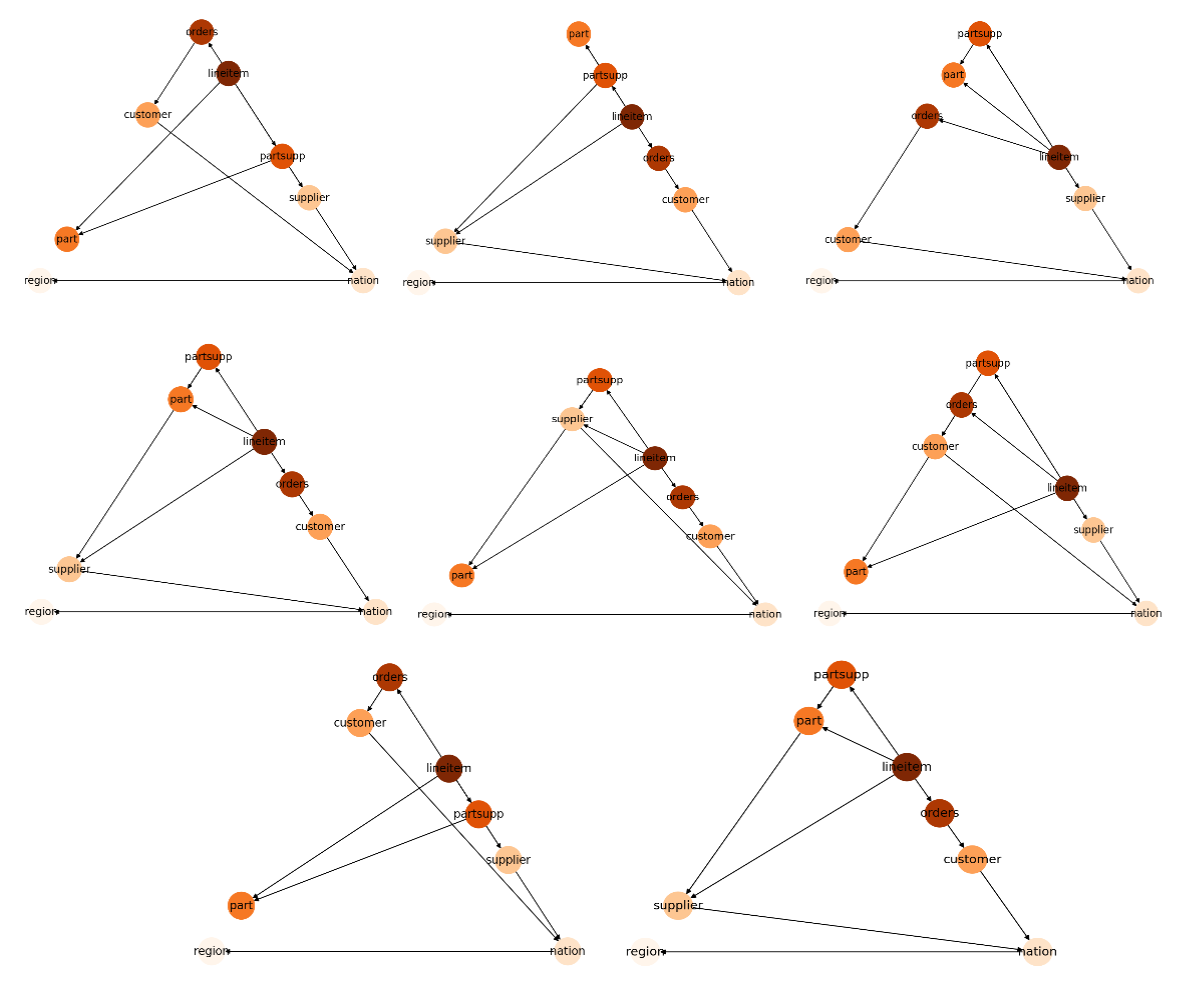
\includegraphics[scale=0.4]{Graphics/jointreesexp2.png}
  \caption{\'Arboles de join para el esquema de TPCH}
  \label{fig:jointree2}
\end{figure}

\subsubsection{Fase 3: Generaci\'on de las consultas}

Los joins computados para la poblaci\'on de cada una de las tablas del esquema estrella del almacén de datos 
\textbf{tpch\_dw} presente en el script del DSL \textbf{tpch.tex} son los siguientes: 

\begin{lstlisting}[label={joinsexp2}, caption={Joins computados para el experimento 2}, language={sql}]
  -- Joins for supplier
  1: supplier JOIN nation ON supplier.s_nationkey = nation.n_nationkey 
     JOIN region ON nation.n_regionkey = region.r_regionkey

  2: lineitem JOIN orders ON lineitem.l_orderkey = orders.o_orderkey 
    JOIN customer ON orders.o_custkey = customer.c_custkey 
    JOIN nation ON customer.c_nationkey = nation.n_nationkey 
    JOIN region ON nation.n_regionkey = region.r_regionkey 
    JOIN partsupp ON lineitem.l_suppkey = partsupp.ps_suppkey AND lineitem.l_partkey = partsupp.ps_partkey 
    JOIN supplier ON partsupp.ps_suppkey = supplier.s_suppkey

  3: lineitem JOIN supplier ON lineitem.l_suppkey = supplier.s_suppkey 
    JOIN orders ON lineitem.l_orderkey = orders.o_orderkey 
    JOIN customer ON orders.o_custkey = customer.c_custkey 
    JOIN nation ON customer.c_nationkey = nation.n_nationkey 
    JOIN region ON nation.n_regionkey = region.r_regionkey

  -- Joins for part
  1: part

  -- Joins for order_date
  1: orders

  -- Joins for lineitem
  1: lineitem JOIN orders ON lineitem.l_orderkey = orders.o_orderkey 
     JOIN partsupp ON lineitem.l_suppkey = partsupp.ps_suppkey AND lineitem.l_partkey = partsupp.ps_partkey 
     JOIN part ON partsupp.ps_partkey = part.p_partkey

  2: lineitem JOIN part ON lineitem.l_partkey = part.p_partkey 
     JOIN orders ON lineitem.l_orderkey = orders.o_orderkey 
     JOIN partsupp ON lineitem.l_suppkey = partsupp.ps_suppkey AND lineitem.l_partkey = partsupp.ps_partkey
\end{lstlisting}

Para el caso de \textbf{part} y \textbf{orders} no es necesario un join por tanto todos los datos se obtienen de 
una sola tabla. 

Seleccionando en todos los casos el primer join mostrado en el listado de c\'odigo \ref{joinsexp2} se generan 
las consultas de creaci\'on mostradas en el listado c\'odigo \ref{genquery2} y las consultas de selecci\'on 
mostradas en el listado de c\'odigo \ref{selectexp2}: 

\begin{lstlisting}[label={genquery2}, caption={Consultas de creaci\'on generadas para el experimento 2}, language={sql}]
  -- Creation query's
  CREATE TABLE IF NOT EXISTS lineitem (
  lnumber serial, 
  partkey INT, 
  supplierkey INT, 
  order_date DATE, 
  totalpayment FLOAT, 
  totalquantity INT, 
  earnings NUMERIC, 
  PRIMARY KEY (lnumber), 
  FOREIGN KEY (partkey) REFERENCES part (p_partkey), 
  FOREIGN KEY (supplierkey) REFERENCES supplier (suppkey), 
  FOREIGN KEY (order_date) REFERENCES order_date (o_date), 
  UNIQUE(partkey, supplierkey, order_date)
  );

  CREATE TABLE IF NOT EXISTS order_date (
  o_date DATE, 
  day TEXT, 
  month TEXT, 
  PRIMARY KEY (o_date)
  );

  CREATE TABLE IF NOT EXISTS part (
  p_partkey INT, 
  name TEXT, 
  brand TEXT, 
  p_size INT, 
  p_retailprice NUMERIC, 
  PRIMARY KEY (p_partkey)
  );

  CREATE TABLE IF NOT EXISTS supplier (
  suppkey INT, 
  name TEXT, 
  phone TEXT, 
  address TEXT, 
  nation TEXT, 
  region TEXT, 
  PRIMARY KEY (suppkey)
  );

  -- level metadata 
  CREATE TABLE IF NOT EXISTS level_metadata (
                                  table_name TEXT,
                                  attribute_name TEXT,
                                  level INT,
                                  PRIMARY KEY (table_name, attribute_name, level));

  INSERT INTO level_metadata VALUES('supplier', 'suppkey', 0);
  INSERT INTO level_metadata VALUES('supplier', 'name', 0);
  INSERT INTO level_metadata VALUES('supplier', 'phone', 0);
  INSERT INTO level_metadata VALUES('supplier', 'address', 0);
  INSERT INTO level_metadata VALUES('supplier', 'nation', 0);
  INSERT INTO level_metadata VALUES('supplier', 'region', 1);
  INSERT INTO level_metadata VALUES('part', 'p_partkey', 0);
  INSERT INTO level_metadata VALUES('part', 'name', 0);
  INSERT INTO level_metadata VALUES('part', 'brand', 0);
  INSERT INTO level_metadata VALUES('part', 'p_size', 0);
  INSERT INTO level_metadata VALUES('part', 'p_retailprice', 0);
  INSERT INTO level_metadata VALUES('order_date', 'o_date', 0);
  INSERT INTO level_metadata VALUES('order_date', 'day', 0);
  INSERT INTO level_metadata VALUES('order_date', 'month', 1);
  INSERT INTO level_metadata VALUES('lineitem', 'lnumber', 0);
  INSERT INTO level_metadata VALUES('lineitem', 'partkey', 0);
  INSERT INTO level_metadata VALUES('lineitem', 'supplierkey', 0);
  INSERT INTO level_metadata VALUES('lineitem', 'order_date', 0);
  INSERT INTO level_metadata VALUES('lineitem', 'totalpayment', 0);
  INSERT INTO level_metadata VALUES('lineitem', 'totalquantity', 0);
  INSERT INTO level_metadata VALUES('lineitem', 'earnings', 0);
\end{lstlisting}

\begin{lstlisting}[label={selectexp2}, caption={Consultas de selecci\'on generadas para el experimento 2}, language={sql}]
  -- Selection for lineitem
  SELECT DISTINCT lineitem.l_partkey AS partkey, lineitem.l_suppkey AS supplierkey, orders.o_orderdate AS order_date, SUM(lineitem.l_payment) AS totalpayment, SUM(lineitem.l_quantity) AS totalquantity, SUM(lineitem.l_payment)-(SUM(lineitem.l_quantity)*partsupp.ps_supplycost)-(SUM(lineitem.l_quantity)*part.p_retailprice) AS earnings
  FROM lineitem
  JOIN orders ON lineitem.l_orderkey = orders.o_orderkey
  JOIN partsupp ON lineitem.l_suppkey = partsupp.ps_suppkey AND lineitem.l_partkey = partsupp.ps_partkey
  JOIN part ON partsupp.ps_partkey = part.p_partkey
  GROUP BY lineitem.l_partkey,lineitem.l_suppkey,orders.o_orderdate,partsupp.ps_supplycost,part.p_retailprice;

  -- Selection for order_date
  SELECT DISTINCT orders.o_orderdate AS o_date, to_char(orders.o_orderdate, 'Day') AS day, to_char(orders.o_orderdate, 'Month') AS month
  FROM orders;

  -- Selection for part 
  SELECT DISTINCT part.p_partkey, part.p_name AS name, part.p_brand AS brand, part.p_size, part.p_retailprice
  FROM part;

  -- Selection for supplier 
  SELECT DISTINCT supplier.s_suppkey AS suppkey, supplier.s_name AS name, supplier.s_phone AS phone, supplier.s_address AS address, nation.n_name AS nation, region.r_name AS region
  FROM supplier
  JOIN nation ON supplier.s_nationkey = nation.n_nationkey
  JOIN region ON nation.n_regionkey = region.r_regionkey;
\end{lstlisting}

\subsubsection{Fase 4: Creaci\'on manual del pipeline y poblaci\'on del almac\'en de datos}

El pipeline creado se encuentra en la ruta \textbf{experiments/tpch} con el nombre de 
\textbf{pipeline.py}. 

La figura \ref{fig:fullpg2} muestra el estado del servidor de bases de datos \textbf{target} luego de la ejecuci\'on 
del pipeline, y nuevamente se puede constatar la correcta poblaci\'on del almac\'en de datos \textbf{tpch\_dw}.

\begin{figure}
  \centering
  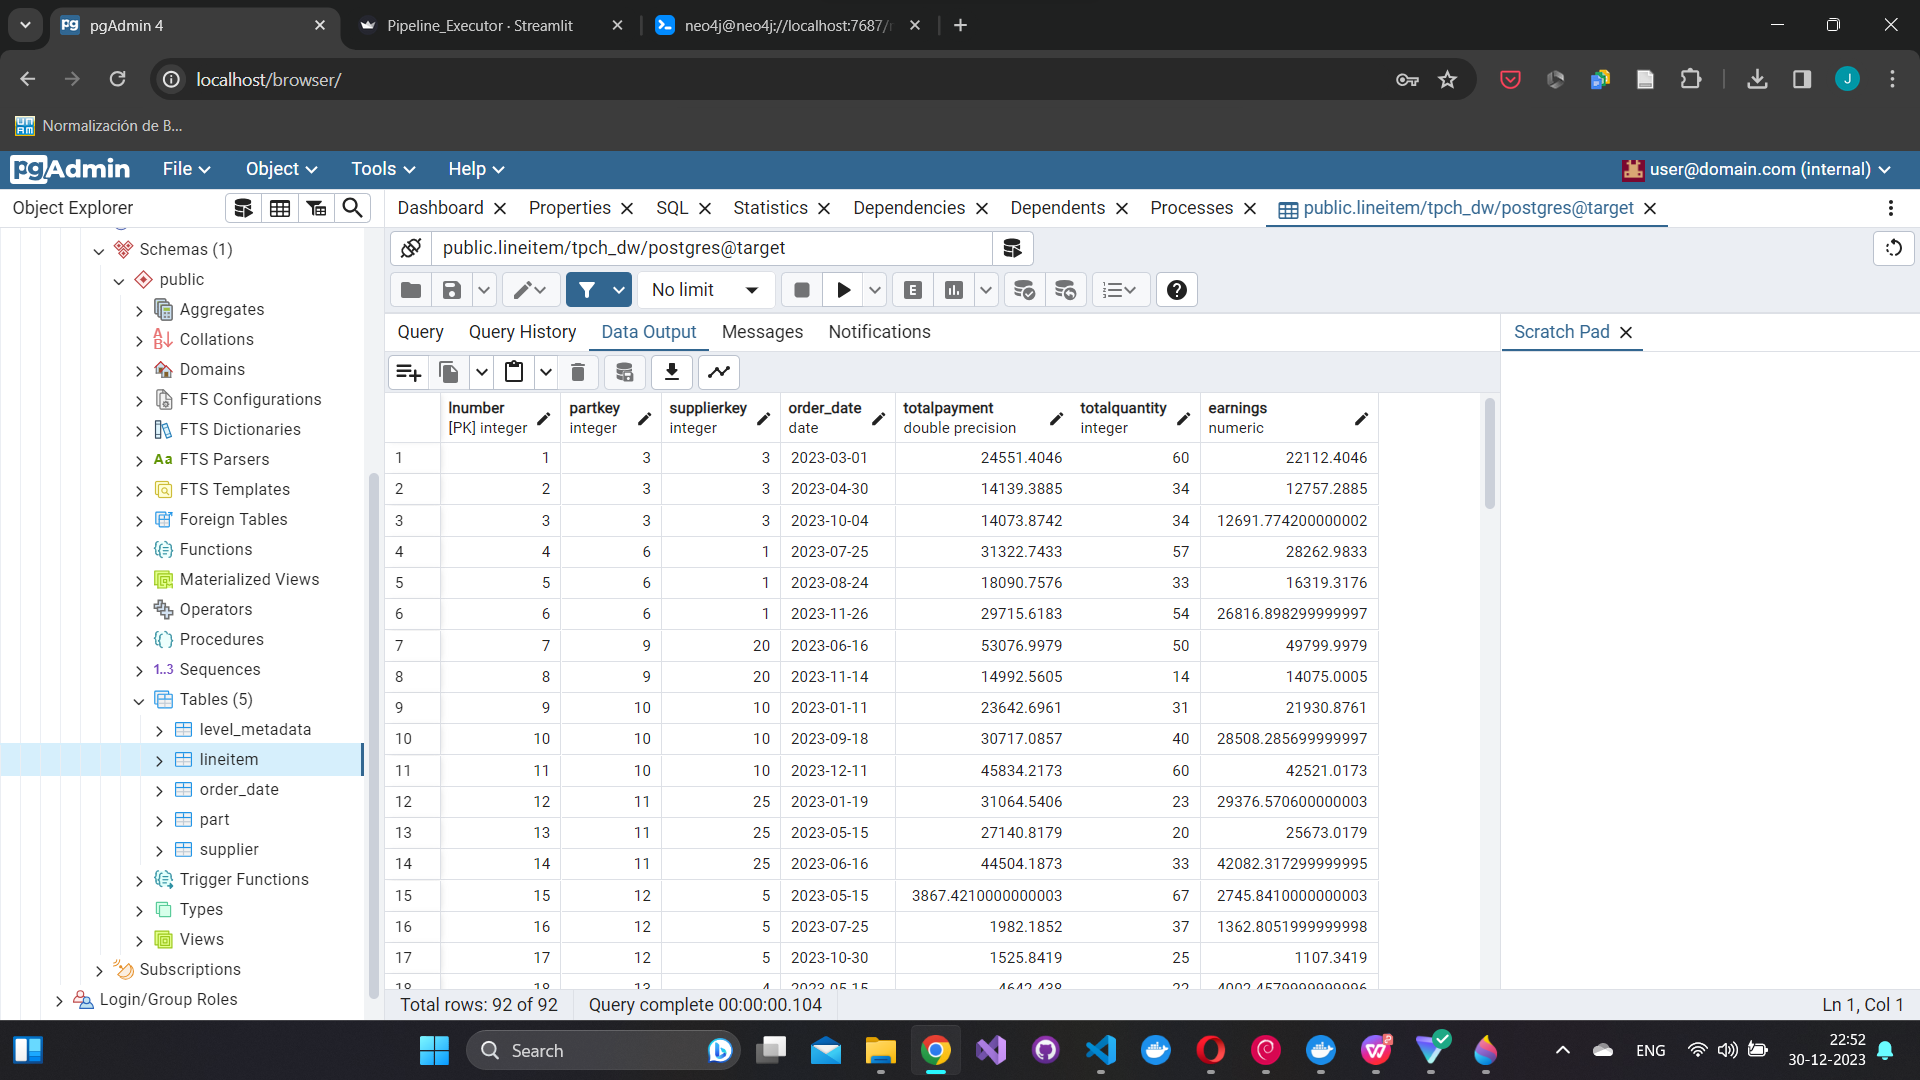
\includegraphics[scale=0.4]{Graphics/fullpgadmin2.png}
  \caption{Almacén de datos poblado asociado al escenario de TPCH}
  \label{fig:fullpg2}
\end{figure}


